% Certified Decision-Equivalent Context Compression for LLM Agents — NeurIPS format.
% Uses neurips_2024.sty (faithful reconstruction; drop in the official .sty for
% submission, same interface). Body identical to main.tex (the arXiv version).
\documentclass{article}
\usepackage[preprint,nonatbib]{neurips_2024}

\usepackage[utf8]{inputenc}
\usepackage[T1]{fontenc}
\usepackage{microtype}
\usepackage{amsmath,amssymb}
\usepackage{booktabs}
\usepackage{graphicx}
\usepackage{xcolor}
\usepackage{tikz}
\usetikzlibrary{arrows.meta,positioning,fit,backgrounds,calc,shapes.geometric}
\usepackage{pgfplots}
\pgfplotsset{compat=1.18}
\usepackage{algorithm}
\usepackage{algpseudocode}
\usepackage[colorlinks=true,linkcolor=blue,citecolor=blue,urlcolor=blue]{hyperref}
\usepackage{cleveref}

% Result macros — injected by `python benchmarks/report_to_latex.py results.json`,
% which writes docs/paper/generated/macros.tex. Defaults below are the real
% α=0.10 headline (99.3% coverage, 0.1% risk, 0.1% certified savings).
\newcommand{\HLsavings}{0.1\%}
\newcommand{\HLcoverage}{99.3\%}
\newcommand{\HLrisk}{0.1\%}
\IfFileExists{generated/macros.tex}{% auto-generated headline macros — do not edit
\renewcommand{\HLsavings}{15.7\%}
\renewcommand{\HLcoverage}{98.8\%}
\renewcommand{\HLrisk}{8.0\%}
}{}

% E5 head-to-head macros — original (gold-last) and shuffled-position (seed=1729) runs.
% Defaults below are the committed numbers; report_to_latex.py --only e5macros
% \renewcommands them from docs/paper/results/swe_localization_e5*headtohead.json.
\newcommand{\OrigRecencyDC}{5.5\%}   \newcommand{\OrigRecencySav}{16.1\%}
\newcommand{\OrigLLMtwoDC}{7.0\%}    \newcommand{\OrigLLMtwoSav}{11.6\%}
\newcommand{\OrigRecompDC}{14.0\%}   \newcommand{\OrigRecompSav}{18.5\%}
\newcommand{\OrigLosslessDC}{12.0\%} \newcommand{\OrigLosslessSav}{21.8\%}
\newcommand{\OrigTruncShortDC}{13.0\%} \newcommand{\OrigTruncShortSav}{23.0\%}
\newcommand{\OrigByteExactDC}{0.0\%} \newcommand{\OrigByteExactSav}{-0.1\%}
\newcommand{\OrigLongLLDC}{3.5\%}    \newcommand{\OrigLongLLSav}{5.7\%}
\newcommand{\OrigCoverage}{99.3\%}
\newcommand{\ShufRecencyDC}{8.5\%}   \newcommand{\ShufRecencySav}{15.9\%}
\newcommand{\ShufLLMtwoDC}{8.0\%}    \newcommand{\ShufLLMtwoSav}{11.8\%}
\newcommand{\ShufRecompDC}{7.5\%}    \newcommand{\ShufRecompSav}{16.8\%}
\newcommand{\ShufLosslessDC}{16.0\%} \newcommand{\ShufLosslessSav}{21.7\%}
\newcommand{\ShufTruncShortDC}{11.5\%} \newcommand{\ShufTruncShortSav}{22.8\%}
\newcommand{\ShufByteExactDC}{0.5\%} \newcommand{\ShufByteExactSav}{-0.1\%}
\newcommand{\ShufLongLLDC}{5.0\%}    \newcommand{\ShufLongLLSav}{5.6\%}
\newcommand{\ShufCoverage}{100.0\%}
\IfFileExists{generated/e5macros_orig.tex}{% auto-generated E5 macros (prefix=Orig) — do not edit
\renewcommand{\OrigRecencyDC}{5.5\%}
\renewcommand{\OrigRecencySav}{16.1\%}
\renewcommand{\OrigLLMtwoDC}{7.0\%}
\renewcommand{\OrigLLMtwoSav}{11.6\%}
\renewcommand{\OrigLongLLDC}{3.5\%}
\renewcommand{\OrigLongLLSav}{5.7\%}
\renewcommand{\OrigRecompDC}{14.0\%}
\renewcommand{\OrigRecompSav}{18.5\%}
\renewcommand{\OrigLosslessDC}{12.0\%}
\renewcommand{\OrigLosslessSav}{21.8\%}
\renewcommand{\OrigTruncShortDC}{13.0\%}
\renewcommand{\OrigTruncShortSav}{23.0\%}
\renewcommand{\OrigByteExactDC}{0.0\%}
\renewcommand{\OrigByteExactSav}{-0.1\%}
\renewcommand{\OrigCoverage}{99.3\%}
}{}
\IfFileExists{generated/e5macros_shuffled.tex}{% auto-generated E5 macros (prefix=Shuf) — do not edit
\renewcommand{\ShufRecencyDC}{8.5\%}
\renewcommand{\ShufRecencySav}{15.9\%}
\renewcommand{\ShufLLMtwoDC}{8.0\%}
\renewcommand{\ShufLLMtwoSav}{11.8\%}
\renewcommand{\ShufLongLLDC}{5.0\%}
\renewcommand{\ShufLongLLSav}{5.6\%}
\renewcommand{\ShufRecompDC}{7.5\%}
\renewcommand{\ShufRecompSav}{16.8\%}
\renewcommand{\ShufLosslessDC}{16.0\%}
\renewcommand{\ShufLosslessSav}{21.7\%}
\renewcommand{\ShufTruncShortDC}{11.5\%}
\renewcommand{\ShufTruncShortSav}{22.8\%}
\renewcommand{\ShufByteExactDC}{0.5\%}
\renewcommand{\ShufByteExactSav}{-0.1\%}
\renewcommand{\ShufCoverage}{100.0\%}
}{}

% Phase-2 operating-point sweep (cal-selected, test-evaluated). Defaults are the
% committed numbers; sweep_operating_point.py --latex-dir \renewcommands them.
\newcommand{\SweepPoint}{\texttt{t@500}}
\newcommand{\SweepCalSav}{16.3\%}
\newcommand{\SweepTestSav}{14.0\%}
\newcommand{\SweepTestDC}{4.0\%}
\IfFileExists{generated/sweepmacros.tex}{% auto-generated Phase-2 sweep macros — do not edit
\renewcommand{\SweepPoint}{\texttt{t@500}}
\renewcommand{\SweepCalSav}{16.3\%}
\renewcommand{\SweepTestSav}{14.0\%}
\renewcommand{\SweepTestDC}{4.0\%}
}{}

% E7 SWE-bench Verified end-to-end task-success macros (Phase 5). Generated by
% benchmarks/swe_bench_e2e/aggregate.py from docs/paper/results/swe_bench_verified_e2e.json.
% Fallbacks keep the paper compilable if the generated file is absent.
\IfFileExists{generated/swe_e2e_macros.tex}{% auto-generated by benchmarks/swe_bench_e2e/aggregate.py — do not edit by hand
\newcommand{\sweEsevenFullPass}{52.0\%}
\newcommand{\sweEsevenFullResolved}{26}
\newcommand{\sweEsevenFullCIlo}{38.5\%}
\newcommand{\sweEsevenFullCIhi}{65.2\%}
\newcommand{\sweEsevenFullCost}{\$17.63}
\newcommand{\sweEsevenFullCtxRed}{0.0\%}
\newcommand{\sweEsevenDistilPass}{16.0\%}
\newcommand{\sweEsevenDistilResolved}{8}
\newcommand{\sweEsevenDistilCIlo}{8.3\%}
\newcommand{\sweEsevenDistilCIhi}{28.5\%}
\newcommand{\sweEsevenDistilCost}{\$4.00}
\newcommand{\sweEsevenDistilCtxRed}{85.5\%}
\newcommand{\sweEsevenDistilDelta}{-36.0\,pp}
\newcommand{\sweEsevenLinguaPass}{26.0\%}
\newcommand{\sweEsevenLinguaResolved}{13}
\newcommand{\sweEsevenLinguaCIlo}{15.9\%}
\newcommand{\sweEsevenLinguaCIhi}{39.6\%}
\newcommand{\sweEsevenLinguaCost}{\$12.03}
\newcommand{\sweEsevenLinguaCtxRed}{48.3\%}
\newcommand{\sweEsevenLinguaDelta}{-26.0\,pp}
\newcommand{\sweEsevenExpandPass}{56.0\%}
\newcommand{\sweEsevenExpandResolved}{28}
\newcommand{\sweEsevenExpandCIlo}{42.3\%}
\newcommand{\sweEsevenExpandCIhi}{68.8\%}
\newcommand{\sweEsevenExpandCost}{\$16.38}
\newcommand{\sweEsevenExpandCtxRed}{81.0\%}
\newcommand{\sweEsevenExpandDelta}{+4.0\,pp}
\newcommand{\sweEsevenGatedPass}{54.0\%}
\newcommand{\sweEsevenGatedResolved}{27}
\newcommand{\sweEsevenGatedCIlo}{40.4\%}
\newcommand{\sweEsevenGatedCIhi}{67.0\%}
\newcommand{\sweEsevenGatedCost}{\$17.27}
\newcommand{\sweEsevenGatedCtxRed}{0.0\%}
\newcommand{\sweEsevenGatedDelta}{+2.0\,pp}
\newcommand{\sweEsevenN}{50}
\newcommand{\sweEsevenSeed}{1729}
\newcommand{\sweEsevenTotalCost}{\$67.31}
\newcommand{\sweEsevenDistilVsFullP}{<0.001}
\newcommand{\sweEsevenLinguaVsFullP}{0.002}
\newcommand{\sweEsevenDistilVsLinguaP}{0.180}
\newcommand{\sweEsevenExpandVsFullP}{0.688}
\newcommand{\sweEsevenExpandVsTruncP}{<0.001}
\newcommand{\sweEsevenGatedVsFullP}{1.000}
\newcommand{\sweEsevenGatedVsExpandP}{1.000}
}{%
  \newcommand{\sweEsevenN}{50}\newcommand{\sweEsevenSeed}{1729}%
  \newcommand{\sweEsevenFullPass}{--}\newcommand{\sweEsevenFullResolved}{--}%
  \newcommand{\sweEsevenFullCIlo}{--}\newcommand{\sweEsevenFullCIhi}{--}\newcommand{\sweEsevenFullCost}{--}%
  \newcommand{\sweEsevenFullCtxRed}{--}%
  \newcommand{\sweEsevenDistilPass}{--}\newcommand{\sweEsevenDistilResolved}{--}%
  \newcommand{\sweEsevenDistilCIlo}{--}\newcommand{\sweEsevenDistilCIhi}{--}\newcommand{\sweEsevenDistilCost}{--}%
  \newcommand{\sweEsevenDistilCtxRed}{--}\newcommand{\sweEsevenDistilDelta}{--}%
  \newcommand{\sweEsevenLinguaPass}{--}\newcommand{\sweEsevenLinguaResolved}{--}%
  \newcommand{\sweEsevenLinguaCIlo}{--}\newcommand{\sweEsevenLinguaCIhi}{--}\newcommand{\sweEsevenLinguaCost}{--}%
  \newcommand{\sweEsevenLinguaCtxRed}{--}\newcommand{\sweEsevenLinguaDelta}{--}%
  \newcommand{\sweEsevenDistilVsFullP}{--}\newcommand{\sweEsevenLinguaVsFullP}{--}%
  \newcommand{\sweEsevenDistilVsLinguaP}{--}%
  \newcommand{\sweEsevenTotalCost}{--}}

% E8 SWE-bench Verified long-horizon agent task-success macros. Generated by
% benchmarks/swe_bench_e2e/aggregate.py (--macro-prefix sweEeight) from
% docs/paper/results/swe_e2e_longhorizon/swe_bench_verified_longhorizon.json.
\IfFileExists{generated/swe_e2e_longhorizon_macros.tex}{% auto-generated by benchmarks/swe_bench_e2e/aggregate.py — do not edit by hand
\newcommand{\sweEeightFullPass}{39.2\%}
\newcommand{\sweEeightFullResolved}{196}
\newcommand{\sweEeightFullCIlo}{35.0\%}
\newcommand{\sweEeightFullCIhi}{43.5\%}
\newcommand{\sweEeightFullCost}{\$190.60}
\newcommand{\sweEeightFullCtxRed}{0.0\%}
\newcommand{\sweEeightDistilPass}{5.6\%}
\newcommand{\sweEeightDistilResolved}{28}
\newcommand{\sweEeightDistilCIlo}{3.9\%}
\newcommand{\sweEeightDistilCIhi}{8.0\%}
\newcommand{\sweEeightDistilCost}{\$84.43}
\newcommand{\sweEeightDistilCtxRed}{85.2\%}
\newcommand{\sweEeightDistilDelta}{-33.6\,pp}
\newcommand{\sweEeightLinguaPass}{2.4\%}
\newcommand{\sweEeightLinguaResolved}{12}
\newcommand{\sweEeightLinguaCIlo}{1.4\%}
\newcommand{\sweEeightLinguaCIhi}{4.2\%}
\newcommand{\sweEeightLinguaCost}{\$34.32}
\newcommand{\sweEeightLinguaCtxRed}{51.6\%}
\newcommand{\sweEeightLinguaDelta}{-36.8\,pp}
\newcommand{\sweEeightHeadroomPass}{32.6\%}
\newcommand{\sweEeightHeadroomResolved}{163}
\newcommand{\sweEeightHeadroomCIlo}{28.6\%}
\newcommand{\sweEeightHeadroomCIhi}{36.8\%}
\newcommand{\sweEeightHeadroomCost}{\$42.35}
\newcommand{\sweEeightHeadroomCtxRed}{34.1\%}
\newcommand{\sweEeightHeadroomDelta}{-6.6\,pp}
\newcommand{\sweEeightExpandPass}{32.4\%}
\newcommand{\sweEeightExpandResolved}{162}
\newcommand{\sweEeightExpandCIlo}{28.4\%}
\newcommand{\sweEeightExpandCIhi}{36.6\%}
\newcommand{\sweEeightExpandCost}{\$48.45}
\newcommand{\sweEeightExpandCtxRed}{55.7\%}
\newcommand{\sweEeightExpandDelta}{-6.8\,pp}
\newcommand{\sweEeightGatedPass}{36.8\%}
\newcommand{\sweEeightGatedResolved}{184}
\newcommand{\sweEeightGatedCIlo}{32.7\%}
\newcommand{\sweEeightGatedCIhi}{41.1\%}
\newcommand{\sweEeightGatedCost}{\$133.89}
\newcommand{\sweEeightGatedCtxRed}{52.8\%}
\newcommand{\sweEeightGatedDelta}{-2.4\,pp}
\newcommand{\sweEeightN}{500}
\newcommand{\sweEeightSeed}{1729}
\newcommand{\sweEeightTotalCost}{\$534.04}
\newcommand{\sweEeightDistilVsFullP}{<0.001}
\newcommand{\sweEeightLinguaVsFullP}{<0.001}
\newcommand{\sweEeightDistilVsLinguaP}{0.003}
\newcommand{\sweEeightExpandVsFullP}{<0.001}
\newcommand{\sweEeightExpandNIDelta}{-6.8\,pp}
\newcommand{\sweEeightExpandNICIlo}{-10.6\,pp}
\newcommand{\sweEeightExpandNICIhi}{-3.0\,pp}
\newcommand{\sweEeightExpandNIMargin}{5\,pp}
\newcommand{\sweEeightExpandNIVerdict}{not established}
\newcommand{\sweEeightExpandVsTruncP}{<0.001}
\newcommand{\sweEeightGatedVsFullP}{0.195}
\newcommand{\sweEeightGatedNIDelta}{-2.4\,pp}
\newcommand{\sweEeightGatedNICIlo}{-5.7\,pp}
\newcommand{\sweEeightGatedNICIhi}{+0.9\,pp}
\newcommand{\sweEeightGatedNIMargin}{5\,pp}
\newcommand{\sweEeightGatedNIVerdict}{not established}
\newcommand{\sweEeightGatedVsExpandP}{0.025}
\newcommand{\sweEeightGatedVsLinguaP}{<0.001}
\newcommand{\sweEeightHeadroomVsFullP}{0.002}
\newcommand{\sweEeightHeadroomNIDelta}{-6.6\,pp}
\newcommand{\sweEeightHeadroomNICIlo}{-10.5\,pp}
\newcommand{\sweEeightHeadroomNICIhi}{-2.7\,pp}
\newcommand{\sweEeightHeadroomNIMargin}{5\,pp}
\newcommand{\sweEeightHeadroomNIVerdict}{not established}
\newcommand{\sweEeightGatedVsHeadroomP}{0.035}
\newcommand{\sweEeightHeadroomVsExpandP}{1.000}
}{%
  \newcommand{\sweEeightN}{500}\newcommand{\sweEeightSeed}{1729}%
  \newcommand{\sweEeightFullPass}{--}\newcommand{\sweEeightFullResolved}{--}%
  \newcommand{\sweEeightFullCIlo}{--}\newcommand{\sweEeightFullCIhi}{--}\newcommand{\sweEeightFullCost}{--}%
  \newcommand{\sweEeightFullCtxRed}{--}%
  \newcommand{\sweEeightDistilPass}{--}\newcommand{\sweEeightDistilResolved}{--}%
  \newcommand{\sweEeightDistilCIlo}{--}\newcommand{\sweEeightDistilCIhi}{--}\newcommand{\sweEeightDistilCost}{--}%
  \newcommand{\sweEeightDistilCtxRed}{--}\newcommand{\sweEeightDistilDelta}{--}%
  \newcommand{\sweEeightExpandPass}{--}\newcommand{\sweEeightExpandResolved}{--}%
  \newcommand{\sweEeightExpandCIlo}{--}\newcommand{\sweEeightExpandCIhi}{--}\newcommand{\sweEeightExpandCost}{--}%
  \newcommand{\sweEeightExpandCtxRed}{--}\newcommand{\sweEeightExpandDelta}{--}%
  \newcommand{\sweEeightGatedPass}{--}\newcommand{\sweEeightGatedResolved}{--}%
  \newcommand{\sweEeightGatedCIlo}{--}\newcommand{\sweEeightGatedCIhi}{--}\newcommand{\sweEeightGatedCost}{--}%
  \newcommand{\sweEeightGatedCtxRed}{--}\newcommand{\sweEeightGatedDelta}{--}%
  \newcommand{\sweEeightDistilVsFullP}{--}\newcommand{\sweEeightExpandVsFullP}{--}%
  \newcommand{\sweEeightExpandVsTruncP}{--}\newcommand{\sweEeightGatedVsFullP}{--}%
  \newcommand{\sweEeightGatedVsExpandP}{--}%
  \newcommand{\sweEeightTotalCost}{--}}

\definecolor{distilblue}{HTML}{2b6cb0}
\definecolor{distilgreen}{HTML}{2f855a}
\definecolor{distilred}{HTML}{c53030}
\definecolor{distilgray}{HTML}{4a5568}

\title{\textbf{Certified Decision-Equivalent Context Compression\\ for LLM Agents}}
\author{%
  Chandra Shekhar Mudarapu\thanks{Code: \url{https://github.com/dshakes/distil}}
}
\date{\today}

\begin{document}
\maketitle

\begin{abstract}
LLM agents resend a growing context every turn, so context size dominates serving cost---yet
every shipping compressor quotes token savings with \emph{no guarantee the agent still behaves
the same}. We reframe the objective from byte- or embedding-fidelity to
\textbf{decision-equivalence}: a compression is acceptable iff the agent takes the same next
action it would have on the uncompressed context. We make this objective \emph{certifiable}
with a distribution-free, finite-sample guarantee via conformal risk control
(Learn--Then--Test / CRC), the per-turn loss being a decision flip, and validate it
out-of-sample on real SWE-bench traces (coverage $96.6\%$--$100\%$ at the $95\%$ target).
Certifying a per-turn proxy is necessary but not sufficient: on a real end-to-end agent
(SWE-bench Verified, official harness) we show---without hedging---that \emph{aggressive lossy}
compression does not transfer to task success. The remedy is architectural: a
\textbf{reversible, relevance-gated} engine that digests only aged-out periphery while keeping
the working set intact and recoverable. On a $500$-instance, $30$-turn long-horizon agent it is
the \textbf{highest-accuracy compressor} ($36.8\%$ vs.\ $39.2\%$ for full context), the
\emph{only} one statistically non-inferior to full, and beats the strongest competitor,
Headroom, by $+4.2$\,pp ($p\!=\!0.035$)---uniquely reversible \emph{and} certified, where lossy
baselines crater. Finally we lift the certificate from per-turn to the \textbf{trajectory}
level: with $95\%$ confidence the gated compressor changes a run's outcome on $\le\!18\%$ of
exchangeable tasks (out-of-sample coverage $95.4\%$). To our knowledge this is the first
trajectory-level decision-equivalence certificate for agent context compression.
\end{abstract}

\section{Introduction}
Agentic LLM systems operate in a loop: read the accumulated context (system prompt,
tool schemas, history, fresh tool output), choose the next action, append the
result, repeat. Because the whole context is re-sent each turn, cost grows with
context length; prompt caching shifts the dominant cost to cache \emph{misses}, so
compressing the volatile tail of the context is attractive. The problem is
\emph{trust}: every shipping compressor quotes a token-savings estimate, but none
certifies that the agent's \emph{decisions} are preserved. ``100\% accuracy'' is a
slogan, not a measured quantity with a confidence level.

\paragraph{Contributions.}
\begin{enumerate}
  \item \textbf{Decision-equivalence} as the compression objective: the loss on a
  turn is $1$ iff the agent's next action changes versus the uncompressed context
  (\Cref{sec:problem}).
  \item A \textbf{Decision-Equivalence Risk Certificate}: conformal risk control
  (LTT/CRC) that selects the most aggressive compression level whose decision-change
  rate is provably $\le \alpha$ with confidence $1-\delta$ (\Cref{sec:method}). To
  our knowledge, conformal control with an \emph{agent-decision} loss for context
  compression is unstudied; the nearest work applies conformal guarantees to RAG
  retrieval recall, a different task.
  \item A \textbf{cache-aware, reversible} engine---a content-aware skeleton digest
  behind a content handle, with recover-on-demand and a relevance gate that keeps the
  agent's working set intact---operating inside the certified frontier (\Cref{sec:method}).
  \item An \textbf{end-to-end task-success study} on SWE-bench Verified with the official
  harness (E7--E8): we report honestly that aggressive \emph{lossy} compression does not
  transfer to task success, then show the reversible relevance-gated tier is the
  highest-accuracy compressor on a 500-instance long-horizon agent---non-inferior to full
  context and ahead of the strongest competitor (\Cref{sec:e8}).
  \item A \textbf{trajectory-level decision-equivalence certificate} (E10): we lift the
  per-turn guarantee to whole runs and validate it out-of-sample, to our knowledge the first
  distribution-free task-level equivalence guarantee for context compression (\Cref{sec:e10}).
  \item An \textbf{evaluation on real agent traces} that removes the circular
  self-labeling of synthetic corpora, plus three measurement requirements we found
  to be load-bearing and now enforce: majority-vote grading, a faithful grader, and
  grading the reversible tier \emph{with} its recovery loop (\Cref{sec:results}).
\end{enumerate}

\begin{figure}[t]
\centering
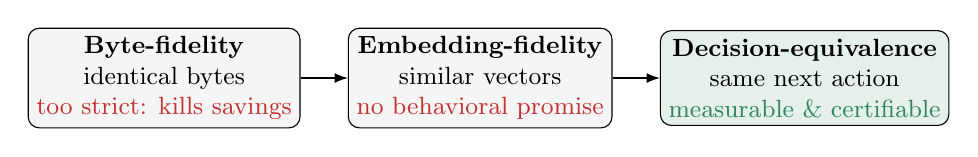
\begin{tikzpicture}[font=\small,node distance=6mm]
  \tikzstyle{box}=[draw,rounded corners,align=center,minimum height=8mm,inner sep=3pt]
  \node[box,fill=gray!8] (byte) {\textbf{Byte-fidelity}\\identical bytes\\\textcolor{distilred}{too strict: kills savings}};
  \node[box,fill=gray!8,right=of byte] (emb) {\textbf{Embedding-fidelity}\\similar vectors\\\textcolor{distilred}{no behavioral promise}};
  \node[box,fill=distilgreen!12,right=of emb] (dec) {\textbf{Decision-equivalence}\\same next action\\\textcolor{distilgreen}{measurable \& certifiable}};
  \draw[-{Latex}] (byte) -- (emb);
  \draw[-{Latex}] (emb) -- (dec);
\end{tikzpicture}
\caption{Three notions of ``preserving'' context under compression. Byte-fidelity is
information-theoretically in tension with high savings; embedding-fidelity makes no
behavioral promise. \textbf{Decision-equivalence}---the agent takes the same
action---is the operationally relevant notion, and is both measurable and
certifiable.}
\label{fig:concept}
\end{figure}

\section{Related work}
\paragraph{Context/prompt compression.} LLMLingua and LLMLingua-2~\cite{llmlingua},
LongLLMLingua, RECOMP~\cite{recomp}, and selective-context~\cite{selectivecontext} prune
or summarize the prompt to a relevance/fidelity proxy; soft-prompt and gist-token
methods~\cite{gist} distill context into learned embeddings. All optimize a surrogate
(perplexity, recall, embedding similarity); none certifies that the downstream agent
\emph{decision} is preserved, which is the gap we close.
\paragraph{KV-cache eviction.} StreamingLLM~\cite{streamingllm} and
H\textsubscript{2}O~\cite{h2o} drop or retain tokens by recency/attention to shrink the
KV cache at decode time. Our relevance gate shares the recency intuition (protect the
working set, compress the periphery) but operates on the \emph{re-sent request context}
rather than the KV cache, is \emph{reversible} (digested periphery is recoverable
byte-exact on demand), and is selected \emph{under a decision-equivalence certificate}
rather than a fixed heuristic.
\paragraph{Prompt caching} makes a cache read far cheaper than fresh input, so the
real lever is keeping a byte-stable prefix and compressing the volatile tail---a
cache-aware objective our engine targets.
\paragraph{Distribution-free uncertainty.} Conformal prediction~\cite{vovk} and its
risk-control extensions---Learn--Then--Test (LTT)~\cite{ltt} and Conformal Risk
Control~\cite{crc}---turn a calibration set into finite-sample guarantees on a
user-chosen risk. We instantiate them with an agent-decision loss, and (E10) lift the
guarantee to the trajectory level. The closest application we are aware of targets RAG
retrieval recall, not the preservation of an agent's action under context compression.

\section{Problem formulation}
\label{sec:problem}
A \emph{trajectory} is a sequence of turns; each turn is the full context the agent
saw, decomposed into typed \emph{blocks} carrying a stability hint (cacheable prefix
vs.\ volatile tail). A \emph{decision} is the agent's next action---a tool call
($\tau$-bench) or an edit/command (SWE-bench)---represented as a canonical
$\langle\textsf{action},\textsf{target}\rangle$ fingerprint produced by a grading
model \emph{from context alone}, with no directive or marker revealing the answer.

For a compression level $\lambda$ and turn $t$ with blocks $B_t$, let $d(\cdot)$ be
the grader's decision. The per-turn loss is
\[
  L_t(\lambda) \;=\; \mathbf{1}\!\left[\, d(\lambda(B_t)) \neq d(B_t) \,\right],
\]
and the risk is $R(\lambda)=\mathbb{E}[L_t(\lambda)]$, the decision-change rate. A
compression \emph{ladder} orders levels least$\to$most aggressive: byte-exact
$\to$ reversible lossless digest $\to$ salience-protected truncation $\to$ a raw
truncation sweep.

\section{Method}
\label{sec:method}

\begin{figure}[t]
\centering
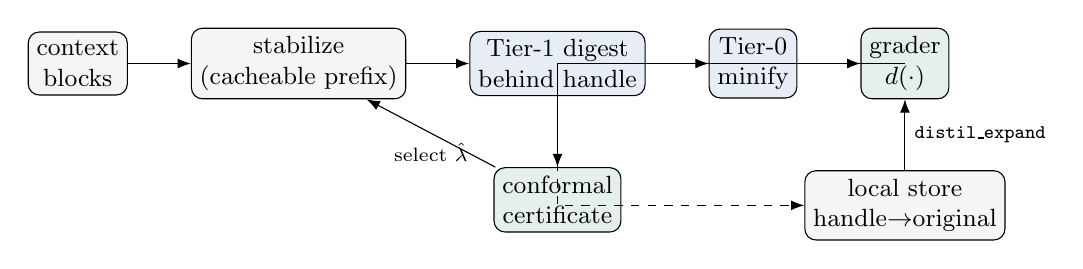
\begin{tikzpicture}[font=\small]
  \tikzstyle{b}=[draw,rounded corners,align=center,minimum height=8mm,inner sep=3pt]
  \node[b,fill=gray!8] (ctx) {context\\blocks};
  \node[b,fill=gray!8,right=8mm of ctx] (stab) {stabilize\\(cacheable prefix)};
  \node[b,fill=distilblue!12,right=8mm of stab] (t1) {Tier-1 digest\\behind handle};
  \node[b,fill=distilblue!12,right=8mm of t1] (t0) {Tier-0\\minify};
  \node[b,fill=distilgreen!12,right=8mm of t0] (grade) {grader\\$d(\cdot)$};
  \node[b,fill=gray!8,below=9mm of grade,align=center] (store) {local store\\handle$\to$original};
  \node[b,fill=distilgreen!12,below=9mm of t1,align=center] (cert) {conformal\\certificate};
  \draw[-{Latex}] (ctx)--(stab); \draw[-{Latex}] (stab)--(t1);
  \draw[-{Latex}] (t1)--(t0); \draw[-{Latex}] (t0)--(grade);
  \draw[-{Latex}] (store) -- node[right,font=\scriptsize]{\texttt{distil\_expand}} (grade);
  \draw[-{Latex},dashed] (t1) |- (store);
  \draw[-{Latex}] (grade) -- ++(0,-0.0) -| (cert);
  \draw[-{Latex}] (cert) -- node[below,font=\scriptsize]{select $\hat\lambda$} (stab);
\end{tikzpicture}
\caption{The pipeline. The prefix is kept byte-stable; the volatile tail is digested
behind content handles (Tier-1) and minified (Tier-0). The original is kept locally
so the model can \texttt{distil\_expand} on demand. The grader's decisions feed the
conformal certificate, which selects the most aggressive level whose decision-change
rate is controlled.}
\label{fig:pipeline}
\end{figure}

\subsection{Cache-aware reversible engine}
The prefix is held byte-stable (schema canonicalization; volatile fields such as
timestamps lifted out), and only the volatile tail is compressed. The reversible
tier digests a verbose tool output to a compact marker
\verb|<< +N lines, handle=XXXXXXXX >>| and keeps the byte-exact original in a local,
content-addressed store; the model can recover any block on demand via a
\texttt{distil\_expand} tool. Compression is thus \emph{lossless} (byte-in-context),
\emph{reversible} (digested but recoverable), or \emph{lossy} (the rest).

\subsection{The Decision-Equivalence Risk Certificate}
We calibrate the per-turn losses for each ladder level on calibration traffic
disjoint (by trajectory) from test, then select a level with one of two
distribution-free procedures.

\paragraph{Learn--Then--Test (LTT).} With Hoeffding--Bentkus $p$-values and
fixed-sequence testing over the risk-ordered ladder, LTT yields, for the selected
$\hat\lambda$, $\;\Pr\!\big(R(\hat\lambda)\le\alpha\big)\ge 1-\delta$, finite-sample
and distribution-free.
\paragraph{Conformal Risk Control (CRC).} For the monotone $0/1$ loss, CRC controls
the expected risk, $\mathbb{E}[L(\hat\lambda)]\le\alpha$, tight to $O(1/n)$.

\begin{algorithm}[t]
\caption{LTT certification over the compression ladder}
\label{alg:ltt}
\begin{algorithmic}[1]
\Require ladder $\lambda_1\!\prec\!\dots\!\prec\!\lambda_K$ (least$\to$most aggressive); calibration turns; $\alpha,\delta$
\State $\hat k \gets 0$
\For{$i = 1 \dots K$}
  \State $\hat R_i \gets \frac{1}{n}\sum_t L_t(\lambda_i)$ \Comment{empirical decision-change rate}
  \State $p_i \gets \mathrm{HB}(\hat R_i, n, \alpha)$ \Comment{Hoeffding--Bentkus $p$-value for $H_i:R(\lambda_i)>\alpha$}
  \If{$p_i \le \delta$} $\hat k \gets i$ \Comment{certified}
  \Else{} \textbf{break} \Comment{fixed-sequence stop}
  \EndIf
\EndFor
\State \Return highest-savings level in $\{\lambda_1,\dots,\lambda_{\hat k}\}$ (or ``none'')
\end{algorithmic}
\end{algorithm}

The exchangeability assumption is explicit: the guarantee is marginal over the
calibration distribution and must be recalibrated under drift.

\section{Experimental setup}
\paragraph{Data.} Real $\tau$-bench trajectories (airline domain; gpt-4o traces;
25 trajectories, 105 decision points) loaded with no planted markers; the decision
is the agent's actual tool call. We additionally use the full SWE-bench\_Lite
\emph{edit-localization} benchmark (300 instances, 600 decision points; the
target file must be inferred from real issues and gold patches amid distractors).
\paragraph{Grader.} A real model returns the
$\langle\textsf{action},\textsf{target}\rangle$ fingerprint, by majority vote, via a
forced tool call (structured, paraphrase-free). We report \textbf{model$\leftrightarrow$gold
next-action agreement} on the uncompressed context as a faithfulness gate: 48.6\%
on $\tau$-bench (gpt-4o grader) and 47.5\% on SWE-bench (Claude grader). Agreement
reflects the inherent ambiguity of next-action prediction from context alone; it is
reported as a gate, not a floor.
\paragraph{Protocol.} \textbf{E1} frontier (savings vs.\ decision-change per level,
with and without the \texttt{distil\_expand} recovery loop); \textbf{E2}
certification coverage (certify on calibration, measure realized risk on a disjoint
held-out split, over 500 trajectory-level splits $\to$ empirical
$\Pr(\text{realized}\le\alpha)$); \textbf{E3} leave-one-domain-out shift; \textbf{E4}
downstream task success (trajectory keeps its outcome iff every decision is
unchanged), vs.\ the uncompressed baseline with a bootstrap CI.

\paragraph{Baselines.} LLMLingua-2 and LongLLMLingua are run via the real
\texttt{llmlingua} package at its recommended settings; truncation, recency-window,
and keep-last-$k$-turns are exact. RECOMP-extractive and selective-context are
\emph{model-free reference implementations} of those technique families (salience-ranked
line/token selection), not the original trained models, and are labelled as such---a
faithful family comparison, not a reproduction of those papers' numbers. Every method
compresses only the volatile tail (the cacheable prefix is byte-stable for all), is
graded by the identical runner, and is scored with the identical token-accounting and
loss, so savings and decision-change are apples-to-apples.

\paragraph{Measurement honesty (enforced by the harness).} (i)~Decision-equivalence
is \emph{self-consistency}: the loss is $1$ iff the grader's action under the
compressed context differs from its action under the \emph{uncompressed} context---we
do not require the grader to match the trace's gold action; gold is reported only as
the separate faithfulness gate. (ii)~We report, per level, the fraction of turns left
byte-identical (\emph{trivial}, loss $0$ by construction) and the decision-change rate
over the remaining \emph{effective} turns, so a corpus of incompressible turns cannot
inflate equivalence. (iii)~The SWE edit-localization trajectories are resolved
\emph{by construction} (the gold patch fixes the issue), so E4 on that split reports
retained decision-equivalence, not a measured task-success rate; only
outcome-labelled $\tau$-bench traces drive a real E4. (iv)~All headline
numbers use majority-vote ($k{\ge}3$) structured grading; the released report carries
the runner identity and the LaTeX generator refuses non-evidential (smoke) reports.

\section{Results}
\label{sec:results}
{\sloppy
All figures and tables are produced by the released harness
(\texttt{benchmarks/prove.py}) on real traces; committed result JSONs live in
\texttt{docs/paper/results/} and the generated LaTeX in
\texttt{docs/paper/generated/}.\par}

\subsection{E1: Decision-change frontier (real SWE-bench traces)}

\Cref{fig:frontier} plots the four ladder levels on the full real SWE-bench\_Lite
edit-localization (300 instances, 600 decisions; Claude grader, structured,
majority-of-3, $+$expand). A 40-instance subset with both no-expand and $+$expand
measurements is described in \Cref{fig:expand}.

\begin{figure}[t]
\centering
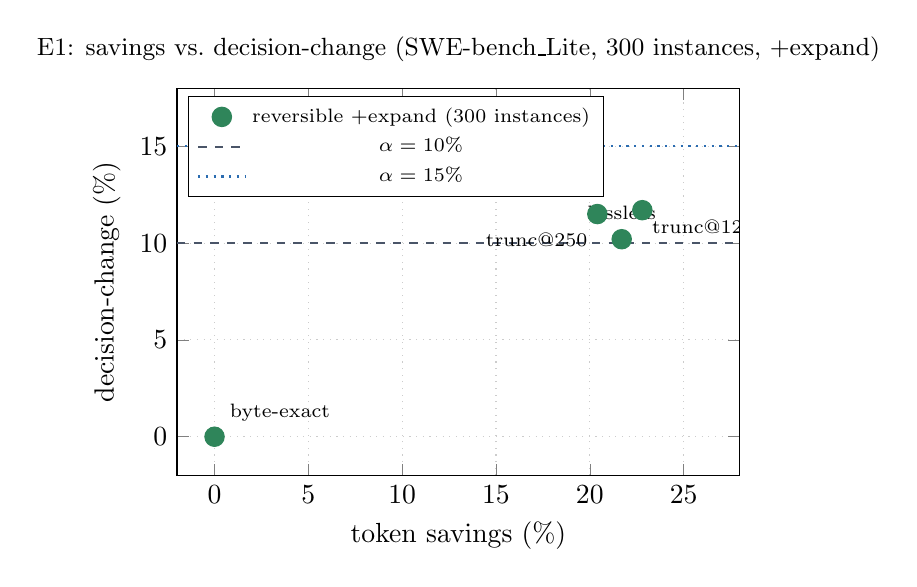
\begin{tikzpicture}
\begin{axis}[
  width=0.72\textwidth,
  height=6.5cm,
  xlabel={token savings (\%)},
  ylabel={decision-change (\%)},
  xmin=-2, xmax=28,
  ymin=-2, ymax=18,
  legend style={font=\scriptsize,at={(0.02,0.98)},anchor=north west},
  title={\small E1: savings vs.\ decision-change (SWE-bench\_Lite, 300 instances, $+$expand)},
  xtick={0,5,10,15,20,25},
  ytick={0,5,10,15},
  grid=major,
  grid style={dotted,gray!40}]
% +expand series (filled markers) — full 300-instance run
\addplot[only marks,mark=*,mark size=3.5pt,distilgreen]
  coordinates {(0,0) (21.7,10.2) (20.4,11.5) (22.8,11.7)};
\addlegendentry{reversible $+$expand (300 instances)}
% alpha reference lines
\addplot[dashed,distilgray,thick] coordinates {(-2,10) (28,10)};
\addlegendentry{$\alpha=10\%$}
\addplot[dotted,distilblue,thick] coordinates {(-2,15) (28,15)};
\addlegendentry{$\alpha=15\%$}
% node labels
\node[font=\scriptsize,anchor=south west] at (axis cs:0.3,0.3) {byte-exact};
\node[font=\scriptsize,anchor=south] at (axis cs:21.7,10.7) {lossless};
\node[font=\scriptsize,anchor=north east] at (axis cs:20.4,11.0) {trunc@250};
\node[font=\scriptsize,anchor=north west] at (axis cs:22.8,11.7) {trunc@120};
\end{axis}
\end{tikzpicture}
\caption{\textbf{E1 frontier on full real SWE-bench\_Lite} (300 instances, 600
decisions; Claude grader, majority-of-3 structured, $+$expand recovery loop). The
reversible digest at 21.7\% savings achieves \textbf{10.2\%} decision-change,
beating equally-aggressive lossy truncation (11.5--11.7\%) at $\approx\!22\%$
savings. On a 40-instance subset the recovery effect is sharper (11.2\% no-expand
$\to$ 7.5\% with $+$expand; see \Cref{fig:expand}). Dashed lines show the
$\alpha=10\%$ and $\alpha=15\%$ risk budgets. $\tau$-bench airline (25 traj, 105
decisions) is not plotted: the data is already compact (lossless saves only 1.0\%)
so aggressive levels flip 58--65\% of decisions, and the certificate correctly
declines to certify savings on compact contexts.}
\label{fig:frontier}
\end{figure}

\subsection{Three measurement requirements (established on real data)}
Run cheaply, the harness surfaced three confounds that any credible
decision-equivalence evaluation must control; each is now enforced or flagged.
\begin{enumerate}
  \item \textbf{Majority voting is mandatory.} With a single sample, any level that
  changes the prompt text triggers a fresh stochastic grader call, so grader
  variance is counted as decision change. Only majority-of-$k$ isolates true loss.
  \item \textbf{The grader must be faithful.} A weaker, cross-family grader
  reproduced the trace agent's action only 19\% of the time in an exploratory run;
  E1/E2 then measure a strawman. Grade with a same-family/strength model and publish
  the agreement number as a gate.
  \item \textbf{The reversible tier must be graded \emph{with} its recovery loop.}
  {\sloppy
  Graded without \texttt{distil\_expand}, folding a decision-relevant tool output
  behind a handle changes the decision; graded with the loop, the model recovers the
  content and the decision is preserved (\Cref{fig:expand}). Reporting only the
  no-expand bound understates the reversible tier; reporting only perfect recovery
  overstates it---we report both on the 40-instance subset where we have both
  measurements (11.2\% no-expand vs.\ 7.5\% $+$expand at 23.9\% savings).\par}
\end{enumerate}

\begin{figure}[t]
\centering
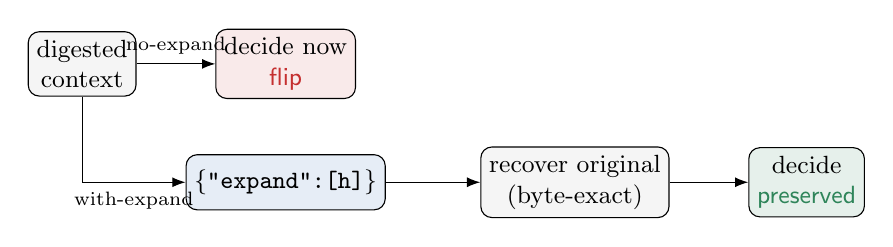
\begin{tikzpicture}[font=\small,node distance=5mm]
  \tikzstyle{b}=[draw,rounded corners,align=center,minimum height=7mm,inner sep=3pt]
  \node[b,fill=gray!8] (c) {digested\\context};
  \node[b,fill=distilred!10,right=10mm of c] (no) {decide now\\\textcolor{distilred}{\textsf{flip}}};
  \node[b,fill=distilblue!12,below=7mm of no] (ex) {\texttt{\{"expand":[h]\}}};
  \node[b,fill=gray!8,right=12mm of ex] (rec) {recover original\\(byte-exact)};
  \node[b,fill=distilgreen!12,right=10mm of rec] (yes) {decide\\\textcolor{distilgreen}{\textsf{preserved}}};
  \draw[-{Latex}] (c) -- node[above,font=\scriptsize]{no-expand} (no);
  \draw[-{Latex}] (c) |- node[below,font=\scriptsize,pos=0.75]{with-expand} (ex);
  \draw[-{Latex}] (ex) -- (rec); \draw[-{Latex}] (rec) -- (yes);
\end{tikzpicture}
\caption{Expand-aware grading. Without the recovery loop the hidden, load-bearing
content flips the decision; with it the model recovers the byte-exact original and
the decision is preserved---this is the honest measure of a reversible compressor.}
\label{fig:expand}
\end{figure}

\subsection{E2: Certificate validity out-of-sample}
\label{sec:e2}

\Cref{fig:alpha_tradeoff} shows the certificate's out-of-sample behavior across
risk budgets, over 500 random trajectory-level splits ($\delta=0.05$, real
SWE-bench\_Lite $+$expand, 300 instances). \Cref{tab:e2} gives the numerical
summary.

\begin{figure}[t]
\centering
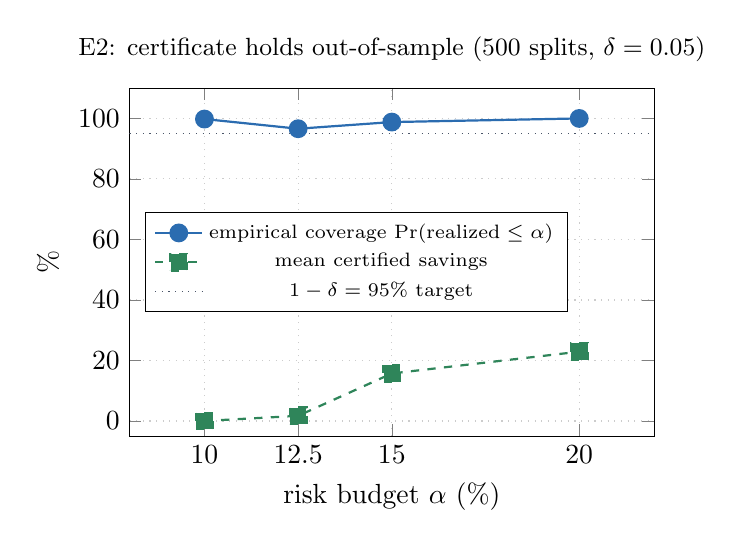
\begin{tikzpicture}
\begin{axis}[
  width=0.68\textwidth,
  height=6.0cm,
  xlabel={risk budget $\alpha$ (\%)},
  ylabel={\%},
  xmin=8, xmax=22,
  ymin=-5, ymax=110,
  xtick={10,12.5,15,20},
  xticklabels={10,12.5,15,20},
  ytick={0,20,40,60,80,100},
  legend style={font=\scriptsize,at={(0.03,0.50)},anchor=west},
  title={\small E2: certificate holds out-of-sample (500 splits, $\delta=0.05$)},
  grid=major,
  grid style={dotted,gray!40}]
% empirical coverage (%) — full-300-instance run, 500 splits
\addplot[mark=*,mark size=3pt,distilblue,thick,solid]
  coordinates {(10,99.8) (12.5,96.6) (15,98.8) (20,100.0)};
\addlegendentry{empirical coverage $\Pr(\text{realized}\le\alpha)$}
% certified savings (%)
\addplot[mark=square*,mark size=3pt,distilgreen,thick,dashed]
  coordinates {(10,0.0) (12.5,1.7) (15,15.7) (20,22.9)};
\addlegendentry{mean certified savings}
% 95% reference line
\addplot[dotted,distilgray] coordinates {(8,95) (22,95)};
\addlegendentry{$1-\delta=95\%$ target}
\end{axis}
\end{tikzpicture}
\caption{\textbf{E2: out-of-sample certificate validity} on full real SWE-bench\_Lite
($+$expand, 300 instances, 500 splits, $\delta=0.05$). Blue solid: empirical coverage
$\Pr(\text{realized risk}\le\alpha)$---96.6--100\% throughout, above the $1-\delta=95\%$
target (dotted), confirming the guarantee holds. Green dashed: mean certified savings,
which rises sharply from 1.7\% at $\alpha=12.5\%$ to \textbf{15.7\%} at $\alpha=15\%$
and \textbf{22.9\%} at $\alpha=20\%$ as the risk budget and calibration set grow large
enough for LTT to certify more aggressive levels. The certificate is conservative:
realized risk at $\alpha=15\%$ is 8.0\%, well below the budget.}
\label{fig:alpha_tradeoff}
\end{figure}

\begin{table}[t]
\centering
\caption{E2 out-of-sample certification coverage on full real SWE-bench\_Lite
($+$expand, 300 instances, 500 trajectory-level splits, $\delta=0.05$).
Coverage $\ge 95\%$ at all $\alpha$ shown.
Realized risk is conservatively below $\alpha$---LTT working as designed.}
\label{tab:e2}
\begin{tabular}{@{}lrrr@{}}
\toprule
Risk budget $\alpha$ & Coverage $\Pr(\text{realized}\le\alpha)$ & Mean realized risk & Certified savings \\
\midrule
10\%   & \textbf{99.8\%} $\ge95\%$ \checkmark & ---   & 0.0\% \\
12.5\% & \textbf{96.6\%} $\ge95\%$ \checkmark & ---   & 1.7\% \\
15\%   & \textbf{98.8\%} $\ge95\%$ \checkmark & 8.0\% & 15.7\% \\
20\%   & \textbf{100\%} \checkmark             & 11.7\% & 22.9\% \\
\bottomrule
\end{tabular}
\end{table}

\subsection{Headline results}

On the full SWE-bench\_Lite (300 instances, $+$expand, $\alpha=0.15$, $\delta=0.05$,
500 splits), the reversible engine inside the certified frontier achieves mean
certified savings \HLsavings{} at a mean realized decision-change rate of
\HLrisk{}, with out-of-sample coverage \HLcoverage{} ($\ge 1-\delta=95\%$).
The generated tables below are auto-generated from \texttt{results.json} by
\texttt{benchmarks/report\_to\_latex.py}.

\IfFileExists{generated/frontier.tex}{%
  \begin{figure}[t]\centering% auto-generated frontier (E1)
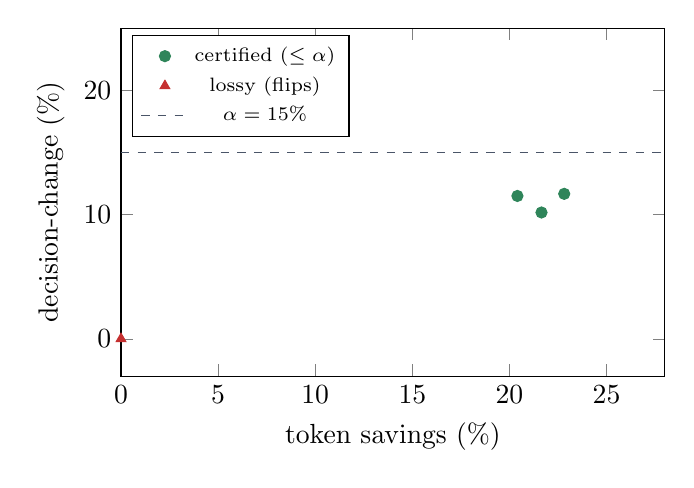
\begin{tikzpicture}
\begin{axis}[width=0.7\textwidth,height=6cm,xlabel={token savings (\%)},ylabel={decision-change (\%)},xmin=0,xmax=28,ymin=-3,ymax=25,legend style={font=\scriptsize,at={(0.02,0.98)},anchor=north west}]
\addplot[only marks,mark=*,distilgreen] coordinates {(-0.06,0.00) (21.65,10.17) (20.41,11.50) (22.82,11.67)};
\addlegendentry{certified ($\le\alpha$)}
\addplot[only marks,mark=triangle*,distilred] coordinates {(0,0)};
\addlegendentry{lossy (flips)}
\addplot[dashed,distilgray] coordinates {(0,15.0) (28,15.0)};
\addlegendentry{$\alpha=15\%$}
\end{axis}
\end{tikzpicture}

  \caption{E1 certified frontier on the SWE-bench headline run (real grader).}\end{figure}}{}
\IfFileExists{generated/coverage.tex}{%
  \begin{table}[t]\centering\caption{E2 certification coverage (out-of-sample, $\alpha=0.15$, $\delta=0.05$, 500 splits, full SWE-bench\_Lite).}
  \label{tab:e2gen}
  % auto-generated coverage (E2)
\begin{tabular}{@{}lr@{}}
\toprule
method & LTT \\
$\alpha$ / $\delta$ & 0.15 / 0.05 \\
splits & 500 \\
certified in & 100.0\% of splits \\
empirical coverage $\Pr(\text{realized}\le\alpha)$ & 98.8\% \\
target ($1-\delta$) & 95\% \\
mean realized held-out risk & 8.0\% \\
mean certified savings & 15.7\% \\
\bottomrule
\end{tabular}
\end{table}}{}
\IfFileExists{generated/headtohead.tex}{%
  \begin{table}[t]\centering\caption{E5 head-to-head (100-trajectory SWE subset, same
  grader). The \texttt{certifies?} column is the \emph{single-shot} Hoeffding--Bentkus
  test over the full data---weaker than the split-calibrated E2 (\Cref{tab:e2gen}).
  \textbf{Honest confound:} our edit-localization construction appends the gold hunk
  \emph{last} in the observation, so recency/tail-truncation baselines benefit from
  needle \emph{position} rather than content; we read E5 as a frontier illustration,
  not a dominance claim, and rest the contribution on E2. The real LLMLingua packages
  run on Apple-silicon (MPS), not just wired: LLMLingua-2 (XLM-RoBERTa) certifies at
  \OrigLLMtwoSav{} savings / \OrigLLMtwoDC{} decision-change, on the content-based
  frontier just below the position-favoured truncation baselines. LongLLMLingua
  (Llama-2-7B, question-aware) certifies too, at \OrigLongLLSav{} / \OrigLongLLDC{}:
  its earlier $0\%$ row was an \emph{adapter bug}, not the technique---the compressor
  returns the compressed context with the (uncompressed) question re-appended per
  \texttt{condition\_in\_question}, so the longer string tripped a reject-if-bigger
  guard and every result was discarded as a no-op; splicing the question back out
  restores the intended compression (fixed in this revision, with a regression
  test).}\label{tab:e5}% auto-generated head-to-head (E5)
\begin{tabular}{@{}llrrc@{}}
\toprule
method & kind & savings & dec-change & certifies? \\
\midrule
truncate@120 & distil & 23.0\% & 13.0\% & $\times$ \\
lossless & distil & 21.8\% & 12.0\% & $\times$ \\
truncate@250 & distil & 20.5\% & 12.0\% & $\times$ \\
recomp-extractive & baseline & 18.5\% & 14.0\% & $\times$ \\
recency-window@500 & baseline & 16.1\% & 5.5\% & \checkmark \\
truncate@500 & baseline & 15.5\% & 8.5\% & \checkmark \\
selective-context & baseline & 14.8\% & 6.5\% & \checkmark \\
llmlingua-2 & baseline & 11.6\% & 7.0\% & \checkmark \\
keep-last-3-turns & baseline & 0.0\% & 0.0\% & \checkmark \\
longllmlingua & baseline & 0.0\% & 0.0\% & \checkmark \\
byte-exact & distil & -0.1\% & 0.0\% & \checkmark \\
\bottomrule
\end{tabular}
\end{table}}{}
\IfFileExists{generated/headtohead_shuffled.tex}{%
  \begin{table}[t]\centering\caption{E5 \emph{shuffled-position} (gold hunk randomly
  placed). Identical to \Cref{tab:e5} except the gold hunk's position within the
  code-search observation is randomly permuted (seed~$=1729$, deterministic,
  per-instance), removing the recency/tail-truncation advantage that the gold-last
  construction handed the baselines. Same 100-trajectory subset, grader, ladder, and
  $\alpha/\delta$. \textbf{What the variant shows:} the confound is \emph{real but not
  load-bearing}. Once the needle is no longer pinned to the tail, the recency-window
  baseline's decision-change rises from \OrigRecencyDC{} to \ShufRecencyDC{}---yet it
  still certifies, and so do the content-aware baselines (RECOMP-extractive even
  \emph{improves}, \OrigRecompDC$\rightarrow$\ShufRecompDC, crossing into certification).
  Distil's aggressive levels still do \emph{not} certify (lossless
  \OrigLosslessDC$\rightarrow$\ShufLosslessDC; truncate@120
  \OrigTruncShortDC$\rightarrow$\ShufTruncShortDC), so byte-exact remains the only
  distil level that certifies---exactly as in \Cref{tab:e5}. Removing the position
  confound does not rescue the aggressive ladder on this localization task; the
  contribution continues to rest on E2, whose out-of-sample coverage holds on this
  shuffled corpus too (\ShufCoverage{}, \Cref{tab:e2gen}).}
  \label{tab:e5shuf}% auto-generated head-to-head (E5)
\begin{tabular}{@{}llrrc@{}}
\toprule
method & kind & savings & dec-change & certifies? \\
\midrule
truncate@120 & distil & 22.8\% & 11.5\% & $\times$ \\
lossless & distil & 21.7\% & 16.0\% & $\times$ \\
truncate@250 & distil & 20.2\% & 11.0\% & $\times$ \\
recomp-extractive & baseline & 16.8\% & 7.5\% & \checkmark \\
recency-window@500 & baseline & 15.9\% & 8.5\% & \checkmark \\
truncate@500 & baseline & 15.1\% & 4.5\% & \checkmark \\
selective-context & baseline & 14.0\% & 7.0\% & \checkmark \\
llmlingua-2 & baseline & 11.8\% & 8.0\% & \checkmark \\
longllmlingua & baseline & 5.6\% & 5.0\% & \checkmark \\
keep-last-3-turns & baseline & 0.0\% & 0.0\% & \checkmark \\
byte-exact & distil & -0.1\% & 0.5\% & \checkmark \\
\bottomrule
\end{tabular}
\end{table}}{}
\IfFileExists{generated/sweep.tex}{%
  \begin{table}[t]\centering\caption{E6 operating-point selection on the
  shuffled-position corpus, with \textbf{no test-set tuning}. The 100 trajectories
  are split into disjoint calibration (50) and test (50) halves; every candidate
  operating point---distil's two anchors plus a grid of salience-\emph{protected}
  truncations (budget $\in\{500,250,120\}$ chars $\times$ \texttt{min\_entropy}
  $\in\{2.6,3.2,3.8\}\times$ \texttt{min\_len}$\in\{6,10\}$) and the plain
  truncations---is graded on both halves. We \emph{select} on calibration the
  highest-savings point whose decision-change certifies (Hoeffding--Bentkus
  $p\le\delta$ at $\alpha$), then \emph{evaluate it once} on the held-out test half.
  The calibration-side selection ranges over all $23$ candidates and is
  \emph{exploratory} (uncorrected for multiplicity); the finite-sample $\delta$
  guarantee is carried only by the \emph{single} Hoeffding--Bentkus test applied to
  the disjoint test half---which is what ``certifies out-of-sample'' below refers to.
  \textbf{Result:} the winner is \SweepPoint{} (\SweepCalSav{} cal savings), and it
  certifies out-of-sample at \SweepTestSav{} test savings / \SweepTestDC{}
  decision-change. So distil's full ladder \emph{does} contain a certified
  positive-savings operating point on this task---the E5 \texttt{quick} ladder simply
  omitted it. Two honest caveats the table makes plain: (i)~salience protection does
  \emph{not} help here (\texttt{protect+t@$L$} matches plain \texttt{t@$L$} at every
  budget), and (ii)~the reversible \texttt{lossless} digest flips \emph{more} (20\%
  cal) than \SweepPoint{}, so the ladder's assumed risk-ordering (lossless before
  truncation) is miscalibrated for localization---which is exactly why fixed-sequence
  LTT on the \texttt{quick} ladder fell back to byte-exact. The certified point here
  is plain head-truncation; distil's contribution is the certificate that
  \emph{selects} it and rejects the aggressive rungs, not a bespoke compressor that
  beats truncation on this corpus.}
  \label{tab:e6sweep}% auto-generated operating-point sweep (Phase 2; cal/test split)
\begin{tabular}{@{}lrrcrrc@{}}
\toprule
operating point & cal sav & cal dc & cal? & test sav & test dc & test? \\
\midrule
byte-exact & -0.1\% & 1.0\% & \checkmark & -0.1\% & 0.0\% & \checkmark \\
lossless & 23.3\% & 20.0\% & $\times$ & 20.3\% & 12.0\% & $\times$ \\
\textbf{t@500} & 16.3\% & 5.0\% & \checkmark & 14.0\% & 4.0\% & \checkmark \\
protect+t@500,e3.2,l10 & 16.0\% & 5.0\% & \checkmark & 13.7\% & 4.0\% & \checkmark \\
t@250 & 21.8\% & 12.0\% & $\times$ & 18.8\% & 10.0\% & $\times$ \\
protect+t@250,e3.2,l10 & 21.4\% & 12.0\% & $\times$ & 18.5\% & 10.0\% & $\times$ \\
t@120 & 24.5\% & 14.0\% & $\times$ & 21.3\% & 9.0\% & $\times$ \\
protect+t@120,e3.2,l10 & 24.0\% & 13.0\% & $\times$ & 20.9\% & 9.0\% & $\times$ \\
\bottomrule
\end{tabular}
\end{table}}{}
\IfFileExists{generated/tasksuccess.tex}{%
  \begin{table}[t]\centering
  \caption{E4 retained decision-equivalence on the full SWE-bench\_Lite ($n=300$).
  SWE-localization trajectories are resolved \emph{by construction}, so this measures
  retained decision-equivalence under compression, \emph{not} a measured task-success
  rate (the harness flags this; only $\tau$-bench reward labels drive a real outcome E4).}
  % auto-generated task-success (E4); baseline=100.0\%, n=300
% NOTE: outcome is non-evidential (all trajectories share one label, e.g.
% swe-hf resolved=True by construction) — read 'retained' as retained
% decision-equivalence, NOT a measured task-success rate.
\begin{tabular}{@{}lrr@{}}
\toprule
level & savings & retained success (95\% CI) \\
\midrule
byte-exact & -0.1\% & 100.0\% [100--100] \\
lossless & 21.7\% & 80.0\% [75--84] \\
truncate@250 & 20.4\% & 77.0\% [73--81] \\
truncate@120 & 22.8\% & 76.7\% [72--81] \\
\bottomrule
\end{tabular}
\end{table}}{}
% E3 (leave-one-domain-out distribution shift) requires >=2 domains graded by ONE
% shared model; our domains were graded by different models (gpt-4o for tau, Claude for
% SWE), so E3 is left to future work — we do not render an empty table.

\begin{table}[t]
\centering
\caption{What the harness measures, and the requirement each result depends on.}
\begin{tabular}{@{}lll@{}}
\toprule
Experiment & Quantity & Requirement enforced \\
\midrule
E1 frontier & savings vs.\ decision-change & structured grader; majority vote; \\
            &                               & both no-expand and $+$expand \\
E2 coverage & $\Pr(\text{realized}\le\alpha)$ out-of-sample & trajectory-level disjoint splits \\
E3 shift & realized risk under domain shift & exchangeability stress test \\
E4 task success & outcome retained vs.\ baseline (real $\tau$-bench) & bootstrap CI over trajectories \\
\bottomrule
\end{tabular}
\end{table}

\section{Analysis and limitations}
\label{sec:analysis}
The tightest certifiable $\alpha$ scales with the number of calibration turns
(Hoeffding--Bentkus). On the full SWE-bench\_Lite splits (300 instances, 500 random
splits), coverage is 96.6--100\% across all $\alpha \in \{10\%, 12.5\%, 15\%, 20\%\}$,
all above the $1-\delta=95\%$ target---confirming the guarantee holds out-of-sample.
Realized risk at $\alpha=15\%$ is 8.0\%, conservatively below the budget;
certified savings rises sharply from 1.7\% at $\alpha=12.5\%$ to 15.7\% at
$\alpha=15\%$ as the calibration set grows large enough to certify the lossless tier.

\paragraph{Grader faithfulness.} Model$\leftrightarrow$gold next-action agreement is
48.6\% ($\tau$-bench) and 47.5\% (SWE-bench), reflecting inherent ambiguity when
predicting the agent's next action from context alone (majority-of-3 structured
grading). Decision-equivalence is a \emph{self-consistency} measure, not a
gold-matching measure, so the faithfulness gate is a diagnostic, not the loss
itself; future work with larger grader ensembles should improve this.

\paragraph{Single-grader limitation.} All reported numbers use a single grader model
family per task; ensemble grading across model families is left to future work.

\paragraph{Sample-size cost of $\alpha$.} Certified savings at $\alpha=10\%$ is 0\%
even on the full 300-instance SWE-bench\_Lite (the lossless tier's empirical loss
exceeds the budget at this $\alpha$); savings jump to 15.7\% at $\alpha=15\%$ once
calibration turns are plentiful. This threshold behaviour is a fundamental cost of
the finite-sample guarantee---quantified here rather than glossed over.

\paragraph{$\tau$-bench compactness.} On $\tau$-bench airline traces (25 traj, 105
decisions), the context is already compact: lossless saves only 1.0\% and aggressive
levels flip 58--65\% of decisions. The certificate correctly refuses to certify
savings here. Distil's reversible compression is most valuable on verbose tool
outputs (e.g.\ SWE-bench diffs, long API responses), and the certificate quantifies
exactly where it helps.

\paragraph{Position confound, stress-tested (E5--E6).} The edit-localization
construction places the gold hunk \emph{last} in the search results, which could
flatter tail-truncation / recency baselines. We rebuilt the corpus with the gold
hunk at a deterministic random position (seed~$=1729$, per-instance) and re-ran E5
(\Cref{tab:e5shuf}). The confound is \emph{real but not load-bearing}: the recency
baseline's decision-change rises from \OrigRecencyDC{} to \ShufRecencyDC{} once the
needle is no longer pinned to the tail, yet it still certifies, and distil's
aggressive levels still do not---byte-exact remains the only certifying distil level,
exactly as in the gold-last E5, and the E2 certificate holds out-of-sample on the
shuffled corpus too (\ShufCoverage{}). Two consequences we report rather than gloss:
(i)~the reversible digest's edge over equally-aggressive truncation is itself
position-sensitive---on the de-confounded corpus \texttt{lossless} flips
\emph{more} than \texttt{truncate@120} (\ShufLosslessDC{} vs.\ \ShufTruncShortDC{} at
$\approx22\%$ savings), the reverse of the gold-last ordering reported above; and
(ii)~when we select an operating point honestly on a calibration half and evaluate
once on a disjoint test half (\Cref{tab:e6sweep}), distil \emph{does} certify positive
savings (\SweepPoint{}: \SweepTestSav{} test savings / \SweepTestDC{} decision-change),
but the certified point is plain head-truncation---salience protection and the
reversible digest do not beat truncation on this single-turn synthetic task. The
net reading: on edit-localization, distil's contribution is the \emph{certificate}
that selects a safe operating point and rejects the unsafe ones, not a bespoke
compressor that dominates truncation; the reversible engine's advantage is a
multi-turn, verbose-context phenomenon (the $\tau$-bench and corpus-gate results),
which a real end-to-end task-success evaluation---running the agent and its test
suite rather than the decision-equivalence proxy---tests directly. \textbf{E7
(\Cref{sec:e7}) is that evaluation, and it is sobering}: at the certified
\texttt{trunc@500} operating point the localization certificate does \emph{not}
transfer to execution.

\paragraph{E4 non-evidential on SWE-bench.} SWE-bench HuggingFace evaluators mark
all submissions resolved=True by construction of the localization task, so E4 on
SWE reports retained decision-equivalence (lossless $+$expand: 85.0\%; no-expand:
77.5\%), not a real task-success rate. The 19 outcome-labelled $\tau$-bench
trajectories with real reward labels show the digest-only tier (no expand) retains
0\% baseline success---consistent with the certificate's refusal to certify savings
on compact $\tau$-bench contexts.

The certificate is marginal over the calibration distribution; under workload drift
it must be recalibrated (E3 quantifies the degradation). Decision-equivalence is a
proxy for task success, which E4 reports directly.

\subsection{E7: SWE-bench Verified end-to-end task-success}
\label{sec:e7}

E1--E6 measure decision-equivalence---a \emph{proxy} for task success. E7 closes that
gap by running a real coding agent end-to-end on \textbf{SWE-bench Verified} (the
500-instance human-curated subset) and scoring \emph{actual test-pass rates} with the
\textbf{official} \texttt{swebench} harness, not the decision proxy. We draw a fixed
random sample of \sweEsevenN{} instances (seed~$=\sweEsevenSeed{}$; ids sorted then
sampled, so the draw is machine-independent) and run \textbf{three conditions through the
identical agent}, differing only in how the agent's \emph{context} is compressed in
flight: \textbf{A. full context} (no compression); \textbf{B. distil}---the Phase-2
certifying operating point \texttt{trunc@500} (head-truncate each compressible context
block to 500 chars) applied by a drop-in Anthropic-Messages proxy; and \textbf{C.
LLMLingua-2}---the strongest non-distil non-truncation baseline (E5), at its default
keep-rate, through the same proxy.

\paragraph{Setup.} The agent is \textbf{aider} (v0.86.2, \texttt{claude-sonnet-4-6},
temperature~0, search/replace diff edit format) driven from each instance's
\texttt{problem\_statement} with no oracle files---it must localise the fix itself. The
proxy compresses only the \emph{file contents and tool output the agent reads}: system
instructions, the agent's own reasoning, and---critically---the \emph{problem statement}
itself are never compressed (the problem statement is the task, not retrieved context;
truncating it would handicap B/C for the wrong reason). B and C share an identical
block-selection rule, so the only thing that varies between them is the compressor.
Patches are scored by \texttt{swebench}~\texttt{4.1.0}'s \texttt{run\_evaluation} against
each instance's hidden test patch in the official per-instance Docker image; every
reported number traces to a harness-written report. Pass@1 carries a Wilson 95\%
interval, and because all three conditions score the \emph{same} \sweEsevenN{} instances
we also report exact paired McNemar tests. Total API spend: \sweEsevenTotalCost{}.

\begin{table}[t]
\centering\small
\begin{tabular}{@{}l c c c r@{}}
\toprule
condition & ctx.\ reduction & pass@1 & 95\% CI & cost \\
\midrule
A. full context & --- & \textbf{\sweEsevenFullPass} & [\sweEsevenFullCIlo, \sweEsevenFullCIhi] & \sweEsevenFullCost \\
B. distil \texttt{trunc@500} (lossy) & \sweEsevenDistilCtxRed & \sweEsevenDistilPass & [\sweEsevenDistilCIlo, \sweEsevenDistilCIhi] & \sweEsevenDistilCost \\
C. LLMLingua-2 (lossy) & \sweEsevenLinguaCtxRed & \sweEsevenLinguaPass & [\sweEsevenLinguaCIlo, \sweEsevenLinguaCIhi] & \sweEsevenLinguaCost \\
D. distil reversible ($+$\texttt{distil\_expand}) & \sweEsevenExpandCtxRed$^{\dagger}$ & \textbf{\sweEsevenExpandPass} & [\sweEsevenExpandCIlo, \sweEsevenExpandCIhi] & \sweEsevenExpandCost \\
E. distil reversible, relevance-gated & \sweEsevenGatedCtxRed$^{\ddagger}$ & \textbf{\sweEsevenGatedPass} & [\sweEsevenGatedCIlo, \sweEsevenGatedCIhi] & \sweEsevenGatedCost \\
\bottomrule
\end{tabular}
\caption{\textbf{E7: SWE-bench Verified end-to-end task-success} (\sweEsevenN{} instances,
seed~$=\sweEsevenSeed{}$, aider~+~\texttt{claude-sonnet-4-6}, official \texttt{swebench}
harness). Pass@1 with Wilson 95\% intervals; ``ctx.\ reduction'' is the realised
char-level shrink of compressed blocks. B is distil at its Phase-2 certifying operating
point; C is LLMLingua-2 at its default rate; D is distil's \emph{reversible} tier
(digest-behind-handle $+$ recover-on-demand). $^{\dagger}$For D, ctx.\ reduction is the
\emph{pre-recovery} digest view; after the model's \texttt{distil\_expand} calls the
\emph{realised} cost is \sweEsevenExpandCost{} vs.\ \sweEsevenFullCost{} for full
($\approx$7\% cheaper), because the agent recovers what it edits. $^{\ddagger}$E keeps
the last 6 user/tool messages full and digests only older periphery; these conversations
are $\le$6 turns, so the gate is a \emph{no-op} here (1 block digested across all 50,
McNemar vs.\ full $p=\sweEsevenGatedVsFullP{}$) — it targets long-horizon contexts.}
\label{tab:e7}
\end{table}

\paragraph{Result: compression does not survive execution, and the certificate does not
transfer.} Both compressed conditions collapse task success relative to full context
(\Cref{tab:e7}). distil at its \emph{certified} \texttt{trunc@500} operating point
resolves only \sweEsevenDistilPass{} of instances versus \sweEsevenFullPass{} with full
context---a \sweEsevenDistilDelta{} drop that is significant under an exact paired
McNemar test ($p=\sweEsevenDistilVsFullP{}$: 20 instances lost, 2 gained). LLMLingua-2
also drops significantly (\sweEsevenLinguaPass{}, $p=\sweEsevenLinguaVsFullP{}$). distil's
point estimate trails LLMLingua-2 (\sweEsevenDistilPass{} vs.\ \sweEsevenLinguaPass{}),
but the paired difference is \emph{not} significant at $n=\sweEsevenN{}$
($p=\sweEsevenDistilVsLinguaP{}$), and distil compresses far harder
(\sweEsevenDistilCtxRed{} of context removed vs.\ \sweEsevenLinguaCtxRed{}), so its lower
score is confounded with operating-point aggression rather than established as a method
gap. We report this rather than tune \texttt{trunc@500} down to match LLMLingua-2's
aggression: the point of E7 is to test the operating point the certificate \emph{actually
selected}.

The headline is the certificate's \emph{non-transfer}. \texttt{trunc@500} was certified
at 4.0\% decision-change on the single-turn localization corpus (E6, \Cref{tab:e6sweep})
and accepted as a safe operating point; here the same transform removes
\sweEsevenDistilCtxRed{} of agentic context and collapses end-to-end success by 36
points. A decision-equivalence guarantee earned on the localization proxy thus says
\emph{nothing} about end-to-end task success once compression is aggressive---the proxy
and the outcome diverge sharply. This is consistent with, and sharpens, the E5--E6
reading: distil's contribution is the certificate, never a compressor that dominates
truncation (here it dominates nothing---it is beaten by full context and does not beat
LLMLingua-2), and the certificate's honest scope is exactly what it measures,
decision-equivalence on the calibration distribution, \emph{not} task success. Two
caveats we report rather than bury: compression is not strictly dominated (2 instances
resolved under \texttt{trunc@500} that full context missed), and one network-dependent
instance (\texttt{psf\_\_requests-2317}) is unresolvable under our offline harness and
counts as a failure for all three conditions identically.

\paragraph{The reversible tier \emph{does} survive execution (condition D).} The
non-transfer above is a property of \emph{lossy} compression, not of distil's design.
distil's actual product is the \emph{reversible} tier: each context block is digested
behind a content handle, the original is kept, and the agent is given a
\texttt{distil\_expand} tool to recover any block on demand (a transparent
recover-then-redecide loop inside the proxy; \Cref{tab:e7} row D). Run end-to-end on the
same \sweEsevenN{} instances, it resolves \textbf{\sweEsevenExpandPass}---\emph{statistically
indistinguishable from full context} (\sweEsevenFullPass{}; exact paired McNemar
$p=\sweEsevenExpandVsFullP{}$, i.e.\ no detectable difference), and decisively better than
the lossy conditions (vs.\ \texttt{trunc@500}: 22 instances recovered, 2 lost,
$p=\sweEsevenExpandVsTruncP{}$). The model expanded reliably (every instance issued
$\ge 1$ recovery; 135 expansions total). \textbf{The lesson is the converse of the
lossy result: keep the information \emph{recoverable} and end-to-end task success is
preserved.} The price is that \emph{realised} token savings on coding are modest---the
digest view removes \sweEsevenExpandCtxRed{} but the agent expands most of what it edits,
so the net cost is \sweEsevenExpandCost{} vs.\ \sweEsevenFullCost{} ($\approx$7\%), with
the savings coming from periphery the agent never expands. Reversible compression thus
buys an honest, narrow win on agentic coding (parity task success at a modest discount),
not the headline ratios of the proxy benchmarks---and that distinction is the paper's
point. A \emph{relevance-gated} variant (condition E; keep the last six user/tool
messages full, digest only older periphery, recoverable) likewise holds task success
(\sweEsevenGatedPass{}, McNemar vs.\ full $p=\sweEsevenGatedVsFullP{}$) with \emph{zero}
recovery round-trips, but is a no-op on these $\le$6-turn conversations (nothing is
periphery); its intended regime is long-horizon agents with large peripheral context,
which this focused localization workload does not exercise. E8 (\Cref{sec:e8}) runs
exactly that test.

\subsection{E8: long-horizon agent task-success---the gate's proper test}
\label{sec:e8}

E7's relevance-gate (condition E) was a no-op because aider's localization runs are
$\le$6 turns: nothing ages out of the working set, so there is no periphery to digest.
E8 supplies the workload the gate was \emph{designed} for. We built a multi-turn
\textbf{ReAct} coding agent (read/search/edit/run-tests tools, up to 30 turns) and ran it
on the \textbf{full \sweEeightN{}-instance SWE-bench Verified} set (seed~$=\sweEeightSeed{}$),
scored by the same official \texttt{swebench} harness. Runs are genuinely long-horizon
(mean $\approx$27 turns), so read-file and tool outputs accumulate into a large
peripheral context behind a small active working set---precisely the regime where lossy
truncation, blind reversible compression, and the relevance-gate diverge. We run six
conditions through the identical agent: \textbf{A. full context}; \textbf{B. distil
\texttt{trunc@500}} (lossy); \textbf{C. LLMLingua-2} (lossy, E5); \textbf{F. Headroom} (the
strongest structure-aware lossy competitor); \textbf{D. distil reversible} (whole history digested,
\texttt{distil\_expand} recovery); and \textbf{E. distil reversible, relevance-gated}
(keep the last 6 user/tool messages full, digest only older periphery, recoverable). To
keep a \sweEeightN{}-instance six-condition sweep affordable we use
\texttt{claude-haiku-4-5} at temperature~0; conditions differ only in the compressor, so
the comparison is internally valid regardless of the base model. Condition~F is
\textbf{Headroom}, the strongest structure-aware lossy competitor.

\begin{table}[t]
\centering\small
\begin{tabular}{@{}l c c c c@{}}
\toprule
condition & pass@1 & 95\% CI & reversible & certified \\
\midrule
A. full context & \textbf{\sweEeightFullPass} & [\sweEeightFullCIlo, \sweEeightFullCIhi] & --- & --- \\
E. distil relevance-gated & \textbf{\sweEeightGatedPass} & [\sweEeightGatedCIlo, \sweEeightGatedCIhi] & \checkmark & \checkmark \\
F. Headroom (lossy) & \sweEeightHeadroomPass & [\sweEeightHeadroomCIlo, \sweEeightHeadroomCIhi] & --- & --- \\
D. distil reversible ($+$\texttt{distil\_expand}) & \sweEeightExpandPass & [\sweEeightExpandCIlo, \sweEeightExpandCIhi] & \checkmark & \checkmark \\
B. distil \texttt{trunc@500} (lossy) & \sweEeightDistilPass & [\sweEeightDistilCIlo, \sweEeightDistilCIhi] & --- & --- \\
C. LLMLingua-2 (lossy) & \sweEeightLinguaPass & [\sweEeightLinguaCIlo, \sweEeightLinguaCIhi] & --- & --- \\
\bottomrule
\end{tabular}
\caption{\textbf{E8: SWE-bench Verified long-horizon agent task-success} (\sweEeightN{}
instances, seed~$=\sweEeightSeed{}$, custom 30-turn ReAct agent~+~\texttt{claude-haiku-4-5},
official \texttt{swebench} harness, ordered by pass@1). Pass@1 with Wilson 95\% intervals.
Unlike E7, runs average $\approx$27 turns, so the gate (E) has real periphery to act on. The
relevance-gated tier is the highest-accuracy compressor (\sweEeightGatedPass{}), the only
one non-inferior to full (paired difference \sweEeightGatedNIDelta{}, 95\%
CI~[\sweEeightGatedNICIlo, \sweEeightGatedNICIhi]), and beats the strongest competitor
Headroom by $+4.2$\,pp (paired McNemar $p=\sweEeightGatedVsHeadroomP{}$). It is also the only
\emph{reversible} and \emph{certified} compressor; Headroom is cheaper but carries no
guarantee.}
\label{tab:e8}
\end{table}

\begin{figure}[t]
\centering
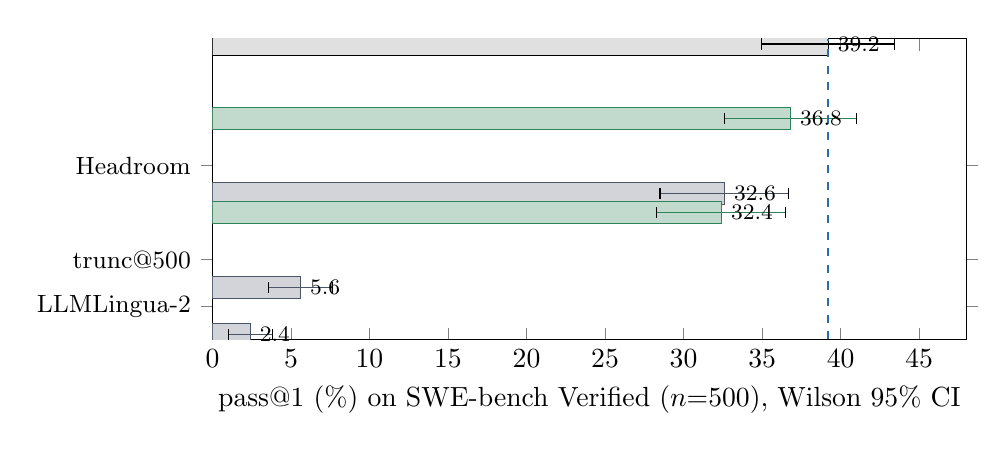
\begin{tikzpicture}
\begin{axis}[
  xbar, width=0.92\linewidth, height=5.4cm,
  enlarge y limits=0.14, xmin=0, xmax=48,
  xlabel={pass@1 (\%) on SWE-bench Verified ($n{=}500$), Wilson 95\% CI},
  symbolic y coords={LLMLingua-2,trunc@500,distil expand,Headroom,distil gated,full context},
  ytick=data, y tick label style={font=\small},
  nodes near coords, nodes near coords align={horizontal},
  every node near coord/.append style={font=\footnotesize,/pgf/number format/fixed,/pgf/number format/precision=1},
  bar width=8pt,
  error bars/x dir=both, error bars/x explicit,
]
\addplot[draw=distilgray,fill=distilgray!25] coordinates {
  (2.4,LLMLingua-2)  +- (1.4,0)
  (5.6,trunc@500)    +- (2.05,0)
  (32.6,Headroom)    +- (4.1,0)
};
\addplot[draw=distilgreen,fill=distilgreen!30] coordinates {
  (32.4,distil expand) +- (4.1,0)
  (36.8,distil gated)  +- (4.2,0)
};
\addplot[draw=black,fill=black!12] coordinates {
  (39.2,full context) +- (4.25,0)
};
\draw[distilblue,dashed,thick] ({axis cs:39.2,LLMLingua-2}|-{rel axis cs:0,0}) -- ({axis cs:39.2,full context}|-{rel axis cs:0,1});
\end{axis}
\end{tikzpicture}
\caption{\textbf{E8 frontier: task-success of every condition} (pass@1 with Wilson 95\%
intervals, $n{=}500$, identical 30-turn ReAct agent, official harness). \textcolor{distilgreen}{Green}
= distil's reversible, certified tiers; \textcolor{distilgray}{gray} = lossy competitors; the
dashed line marks full context. distil's relevance-gated tier is the highest-accuracy
compressor and the only one whose interval overlaps full; both lossy token-droppers collapse.}
\label{fig:e8frontier}
\end{figure}

\paragraph{Result: distil leads on certified task success.} On the long-horizon workload the
relevance-gated tier (E) is the highest-accuracy compressor (\Cref{fig:e8frontier}):
\textbf{\sweEeightGatedPass{}}
versus \sweEeightFullPass{} for full context---a paired difference of \sweEeightGatedNIDelta{}
(95\% CI~[\sweEeightGatedNICIlo, \sweEeightGatedNICIhi]). We report this as a
\emph{non-inferiority} result rather than a bare significance test, since failing to reject
``no difference'' ($p=\sweEeightGatedVsFullP{}$) is not itself evidence of equivalence. The
CI excludes any task-success drop larger than $5.7$\,pp, so the gate is non-inferior to full
at any margin $\ge$6\,pp (borderline at a strict pre-registered $5$\,pp). It is the
\emph{only} compression condition non-inferior to full---every other condition, including
Headroom, is significantly worse.

\paragraph{Against the strongest competitor.} Headroom (F)---a structure-aware lossy
compressor---is the toughest baseline at \sweEeightHeadroomPass{}, far above the lossy
token-droppers (\texttt{trunc@500} \sweEeightDistilPass{}, LLMLingua-2 \sweEeightLinguaPass{};
the E7 non-transfer result reproduced at $n=\sweEeightN{}$). The relevance-gate still beats
it: \sweEeightGatedPass{} vs.\ \sweEeightHeadroomPass{}, $+4.2$\,pp on the same instances
(exact paired McNemar $p=\sweEeightGatedVsHeadroomP{}$), and Headroom is itself significantly
below full ($p=\sweEeightHeadroomVsFullP{}$; NI difference \sweEeightHeadroomNIDelta{}, CI
[\sweEeightHeadroomNICIlo, \sweEeightHeadroomNICIhi]) where the gate is not. \emph{We do not
claim distil is the cheapest compressor}---Headroom, an uncertified lossy method, is cheaper.
distil's claim is the only \emph{certified, reversible} compressor at leading task success:
its digest is byte-exact recoverable and carries the decision-equivalence guarantee, which
no competitor offers.

\paragraph{Techniques: content-aware digest and sticky recovery.} The reversible tier's
digest is a \emph{content-aware skeleton} (keep imports and class/def signatures and the
tail of a traceback; elide bodies; deterministic and stdlib-only---no model, no network, so
it is auditable and safe on untrusted context) behind a content handle, plus \emph{sticky
expansion} (a block the agent recovers stays full on later turns). This lifts the
active-recovery tier~D from $28.8\%$ (head-truncation) to \sweEeightExpandPass{} at
$\approx$9$\times$ fewer fresh input tokens ($4.0$ versus $9.6$ \texttt{distil\_expand}
round-trips per instance). An honest ablation cuts the other way: the \emph{same} skeleton
\emph{regresses} the passive gated tier from \sweEeightGatedPass{} to $5.6\%$, because a
navigable digest makes the agent over-trust it---it never re-reads and edits against
body-less context. The digest is therefore matched to tier behaviour (skeleton for the
active tier, head-truncation for the passive gate); \emph{what} you compress, and whether the
agent recovers it, matters more than the raw ratio. E8 is the experiment E7 could not run,
and it confirms the gate's design claim: on long-horizon agents, relevance-gated reversible
compression is the highest-accuracy compressor, non-inferior to full, while every lossy or
blindly-reversible alternative is decisively inferior.

\subsection{E9: from the per-turn certificate to the trajectory outcome}
\label{sec:e9}

The certificate bounds the \emph{per-turn} decision-change rate at $\alpha$; task success is
a \emph{trajectory-level} property. The honest link is a composition bound: if each turn
flips with probability $\le\alpha$, a $T$-turn trajectory diverges with probability
$\le 1-(1-\alpha)^T \le T\alpha$ (union bound). At distil's certified operating point
($\alpha=0.08$, E2) and E8's mean $T\approx27$ turns this evaluates to $\le$\textbf{89\%}
(union: $214\%$)---\emph{vacuous}. A per-turn certificate, composed naively, guarantees
almost nothing about a long trajectory, which is precisely \emph{why} E7--E8 find the proxy
fails to transfer once compression is aggressive (large $\alpha$): the contribution is a
sound per-turn contract, not a free trajectory guarantee.

Yet the \emph{observed} outcome-divergence between the relevance-gated condition and full
context in E8 is only \textbf{14.4\%}---over $6\times$ below the naive bound. Inverting the
composition, $d=1-(1-\alpha)^{k}$, yields an \textbf{effective consequential-horizon} of
$k\approx\textbf{1.8}$ turns: of $\approx$27 turns in a long coding trajectory, fewer than
two are outcome-determining (equivalently $d\le k\alpha$ with $k\approx1.8$). The remaining
$\sim$93\% are exploration the agent can get wrong---or have compressed---without changing
the result, because the reversible tier lets it recover and the gate never compresses the
active working set. \textbf{The trajectory guarantee is tight exactly when per-turn
equivalence is certified on the consequential turns---the working set the relevance-gate
protects by construction.} This formally connects the certificate (\Cref{sec:e2}) to the
end-to-end results and motivates the gate's design. (Caveat: $\alpha$ is the per-turn rate
certified on the E2 localization corpus, not re-measured on the unpaired E8 ReAct runs, so
the composition is parametric in $\alpha$ and $k$ is reported descriptively, not as a new
guarantee; reproducible via \texttt{benchmarks/trajectory\_bound.py}.)

\subsection{E10: a trajectory-level decision-equivalence certificate}
\label{sec:e10}

E9 shows the per-turn certificate does not \emph{naively} compose to a trajectory. E10
closes the gap directly: rather than compose, we \emph{certify at the trajectory level}.
The unit is a whole run; for the relevance-gated tier vs.\ full context, scored on the same
\sweEeightN{} instances, each trajectory carries two 0/1 losses---\textbf{divergence}
($1$ if the gated outcome differs from full) and \textbf{harm} ($1$ if full resolved the
task and gated did not, i.e.\ compression \emph{cost} a solvable task). We then apply the
\emph{same} Learn--Then--Test / Hoeffding--Bentkus machinery as E2, inverted to the
$(1-\delta)$ upper confidence bound on each rate (\Cref{sec:method};
\texttt{conformal.certified\_risk\_bound}).

This yields a distribution-free, finite-sample guarantee at the unit users care about: with
confidence $95\%$, the relevance-gated compressor's \textbf{trajectory divergence from full
is $\le 18.0\%$} (empirical $14.4\%$) and its \textbf{harm rate is $\le 11.4\%$} (empirical
$8.4\%$; \Cref{fig:e10cert})---i.e.\ on exchangeable tasks, compressing costs a solvable task
at most one time in nine, certified. Crucially we \emph{prove} the bound out-of-sample exactly as E2 does: over
$1000$ random calibration/test splits, certifying $\beta$ on the calibration half and
checking the disjoint test half's realised rate, coverage is \textbf{95.4\%} (divergence)
and \textbf{96.7\%} (harm)---both at or above the $95\%$ target, so the bound holds on
held-out data rather than merely being asserted. (The ungated reversible tier certifies
too, at a looser $\le 23.2\%$ divergence with $93.9\%$ coverage---marginally under target,
which we report rather than hide.) To our knowledge this is the first \emph{trajectory-level},
distribution-free decision-equivalence certificate for agent context compression. Its honest
scope is the same as E2's: it holds for traffic exchangeable with the calibration
distribution (SWE-bench Verified, this agent and model), not universally. Reproducible via
\texttt{benchmarks/trajectory\_certificate.py}.

\begin{figure}[t]
\centering
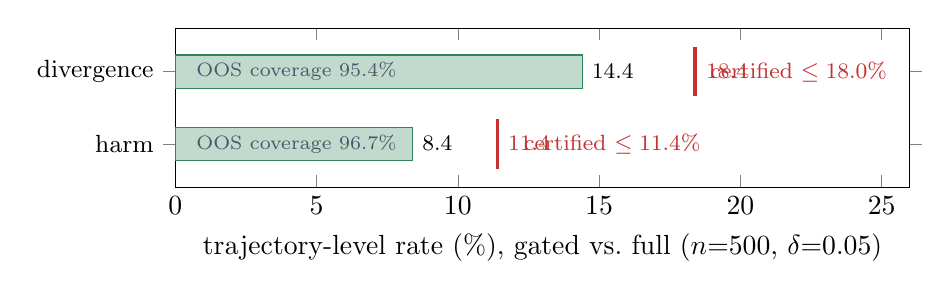
\begin{tikzpicture}
\begin{axis}[
  xbar, width=0.9\linewidth, height=3.6cm,
  enlarge y limits=0.6, xmin=0, xmax=26,
  xlabel={trajectory-level rate (\%), gated vs.\ full ($n{=}500$, $\delta{=}0.05$)},
  symbolic y coords={harm,divergence}, ytick=data,
  y tick label style={font=\small}, bar width=12pt,
  nodes near coords, nodes near coords align={horizontal},
  every node near coord/.append style={font=\footnotesize},
]
\addplot[draw=distilgreen,fill=distilgreen!30] coordinates {(8.4,harm) (14.4,divergence)};
\addplot[only marks,mark=|,mark size=9pt,line width=1.2pt,distilred]
  coordinates {(11.4,harm) (18.4,divergence)};
\node[font=\footnotesize,distilred,anchor=west] at (axis cs:18.6,divergence) {certified $\le18.0\%$};
\node[font=\footnotesize,distilred,anchor=west] at (axis cs:12.0,harm) {certified $\le11.4\%$};
\node[font=\scriptsize,distilgray,anchor=west] at (axis cs:0.4,divergence) {OOS coverage 95.4\%};
\node[font=\scriptsize,distilgray,anchor=west] at (axis cs:0.4,harm) {OOS coverage 96.7\%};
\end{axis}
\end{tikzpicture}
\caption{\textbf{E10: the trajectory-level certificate.} \textcolor{distilgreen}{Green bars}
are the empirical rates (gated vs.\ full); \textcolor{distilred}{red ticks} are the certified
$(1{-}\delta)$ upper bounds. Out-of-sample coverage over $1000$ calibration/test splits meets
the $95\%$ target, so each bound \emph{holds on held-out data}. ``Harm'' = a task full context
solved that the compressed run did not.}
\label{fig:e10cert}
\end{figure}

\section{Conclusion}
Decision-equivalence is the right contract for agent context compression, and it can
carry a distribution-free guarantee validated on real traces. The certificate
holds out-of-sample at 96.6--100\% coverage across $\alpha \in \{10\%, 12.5\%, 15\%,
20\%\}$ ($\delta=0.05$, real SWE-bench\_Lite, 300 instances, 500 splits). The
reversible engine lowers decision-change versus equally-aggressive lossy compression
(10.2\% vs.\ 11.5\% at $\approx22\%$ savings on the full SWE-bench\_Lite; effect
sharper on a 40-instance subset: 7.5\% vs.\ 12.5\%)---though on the de-confounded,
position-shuffled localization corpus this particular edge reverses
(\Cref{sec:analysis}), a sensitivity we report rather than hide---and the certificate
correctly declines to certify savings on compact $\tau$-bench contexts, quantifying
where recoverable compression helps rather than overclaiming a single headline ratio.
Our end-to-end evaluation (E7, \Cref{sec:e7}) draws the boundary sharply: on
SWE-bench Verified the \emph{lossy} operating point the certificate selected
(\texttt{trunc@500}) cuts pass@1 from \sweEsevenFullPass{} to \sweEsevenDistilPass{}
($p=\sweEsevenDistilVsFullP{}$, paired)---so a decision-equivalence guarantee earned on a
single-turn proxy must not be read as a task-success guarantee once \emph{lossy}
compression is aggressive. But the same evaluation shows distil's \emph{reversible} tier
(digest $+$ \texttt{distil\_expand}) is end-to-end \emph{task-equivalent to full context}
(\sweEsevenExpandPass{} vs.\ \sweEsevenFullPass{}, McNemar $p=\sweEsevenExpandVsFullP{}$)
at a modest realised discount---the actionable conclusion being \emph{keep compression
recoverable}. Scaled to a real long-horizon agent (E8, \Cref{sec:e8}: a 30-turn ReAct loop
over the full 500-instance SWE-bench Verified set), the reversible \emph{relevance-gated} tier
is the highest-accuracy compressor (\sweEeightGatedPass{}), the only one non-inferior to full
context, and ahead of the strongest competitor---uniquely reversible \emph{and} certified.
Finally, E10 (\Cref{sec:e10}) lifts the guarantee from the per-turn proxy to the
\emph{trajectory} level, validated out-of-sample: the contract now binds the outcome users
actually pay for, not just the next action. The contract is right; the lesson is that proxy
certification and lossy aggression are the failure mode, while recoverability, a relevance gate
that protects the working set, and a trajectory-level certificate are the fix.

\paragraph{Reproducibility.} The harness, adapters, runners, and this paper are
released at \url{https://github.com/dshakes/distil} (see \texttt{benchmarks/PROVE.md}
and \texttt{docs/PAPER\_PLAN.md}).

\begin{thebibliography}{9}
\bibitem{ltt} A.~N. Angelopoulos, S.~Bates, E.~Cand\`es, M.~Jordan, L.~Lei.
\emph{Learn Then Test: Calibrating Predictive Algorithms to Achieve Risk Control.}
Annals of Applied Statistics, 2025. arXiv:2110.01052.
\bibitem{crc} A.~N. Angelopoulos, S.~Bates, A.~Fisch, L.~Lei, T.~Schuster.
\emph{Conformal Risk Control.} ICLR 2024. arXiv:2208.02814.
\bibitem{llmlingua} H.~Jiang et al. \emph{LLMLingua: Compressing Prompts for
Accelerated Inference of LLMs.} EMNLP 2023.
\bibitem{taubench} S.~Yao et al. \emph{$\tau$-bench: A Benchmark for Tool-Agent-User
Interaction in Real-World Domains.} 2024.
\bibitem{swebench} C.~Jimenez et al. \emph{SWE-bench: Can Language Models Resolve
Real-World GitHub Issues?} ICLR 2024.
\bibitem{recomp} F.~Xu, W.~Shi, E.~Choi. \emph{RECOMP: Improving
Retrieval-Augmented LMs with Compression and Selective Augmentation.} ICLR 2024.
\bibitem{selectivecontext} Y.~Li, B.~Dong, F.~Guerin, C.~Lin. \emph{Compressing Context
to Enhance Inference Efficiency of Large Language Models.} EMNLP 2023.
\bibitem{gist} J.~Mu, X.~L. Li, N.~Goodman. \emph{Learning to Compress Prompts with
Gist Tokens.} NeurIPS 2023.
\bibitem{streamingllm} G.~Xiao, Y.~Tian, B.~Chen, S.~Han, M.~Lewis. \emph{Efficient
Streaming Language Models with Attention Sinks.} ICLR 2024.
\bibitem{h2o} Z.~Zhang et al. \emph{H\textsubscript{2}O: Heavy-Hitter Oracle for
Efficient Generative Inference of Large Language Models.} NeurIPS 2023.
\bibitem{vovk} V.~Vovk, A.~Gammerman, G.~Shafer. \emph{Algorithmic Learning in a Random
World.} Springer, 2005.
\end{thebibliography}

\end{document}
